As was briefly mentioned in the introduction, a number of different paradigms
exist for undertaking computing tasks too resource intensive for a single
commodity computer. These paradigms are discussed in detail below:

\begin{enumerate}
  \item \underline{Supercomputing}: The supercomputing model responds to
    increased demands for computing resources by increasing the technical
    specifications of the computer far beyond the range of the
    traditional commodity PC.
    While supercomputers are able to avoid the majority of the complications
    resulting from the introduction of networks, most prominently reliability and
    security, there are naturally limits on the power of supercomputers.
    Importantly, constructing supercomputers is extremely expensive, and thus
    their computing power is not available to the general public. Furthermore,
    it is difficult to scale a supercomputer should the need arise. Finally,
    supercomputers offer a single point of failure, meaning they are not
    particularly robust to error. These limitations have decreased the usage of
    supercomputers to provide the mass of computing power needed in the ``Big
    Data'' era.

  \item \underline{Cluster Computing}: Cluster computing is defined as utilizing
    ``a collection of similar workstations of PCs, losely connected by means of
    a high-speed local-area network [where] each node runs the same operating
    system.''\cite[pg. 17-18]{distributed-systems-principles-and-paradigms}
    Cluster computing can provide a mass of computing power similar to
    that contained in a supercomputer. Cluster computing also offers many
    advantages over the single supercomputer. First, and perhaps most
    importantly, they are much more cost-efficient, and thus much more
    accessible. Second, clusters are easy to
    scale by simply adding new commodity PCs as nodes.
    Finally, cluster computing is much more fault
    tolerant, as a single failing commodity computer will simply be removed
    from the cluster. Cluster computing is used in the
    implementation of what is colloquially referred to as \textit{Cloud
    computing}, in which large amounts of computing resources are offered on a
    per-usage basis.\cite[pg. 13]{distributed-systems-concepts-and-design}
    Cloud computing, as implemented by Amazon Web
    Services,\cite{amazon-web-services} Microsoft Azure,\cite{microsoft-azure}
    and Google Compute Engine,\cite{google-compute-engine} continue to
    revolutionize the development and deployment of computing applications, as
    developers gain access to cheap, easily accessible, and quickly scalable
    computing power.

    \begin{figure}[!h]
      \centerline{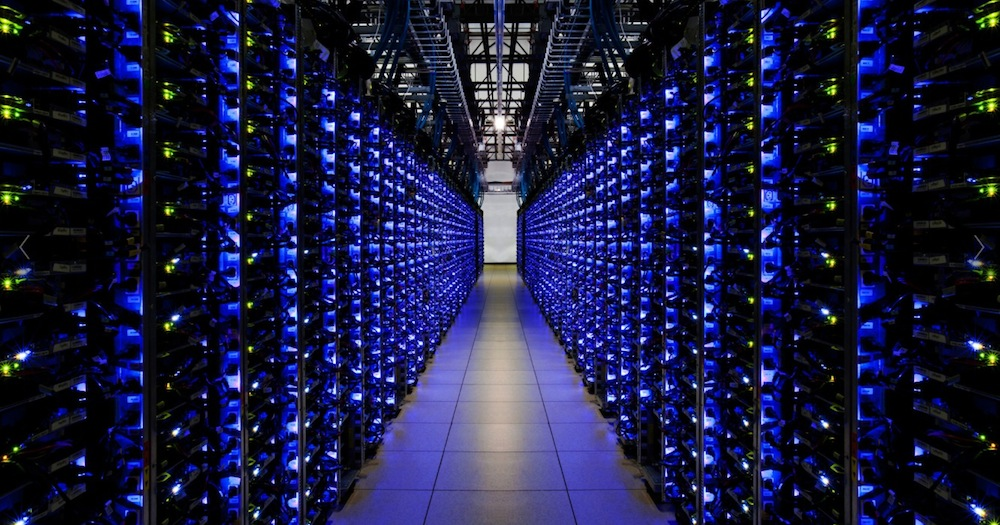
\includegraphics[scale=.4]{google-cluster.jpg}}
      \caption{A Google Computing Cluster.\cite{image-google-cluster}}
    \end{figure}

  \item \underline{Grid Computing}: Grid computing is similar to concept in
    cluster computing, except it foregoes the requirement that all computers
    within the grid be relatively homogeneous. As such, the grid computing model accounts
    for a large degree of heterogeneity with respect to network membership,
    operating system, hardware, and more.\cite[pg.
    18]{distributed-systems-principles-and-paradigms} While grid computing
    systems lack of homogeneity requirements increase flexibility,
    the resulting heterogeneity introduces significant complexity.

\end{enumerate}

Ultimately, because of simplicity, cost, and scalability, cluster computing is
the most prominent resource intensive computing paradigm. Thus, cluster
computing, and the accompanying cluster manager, is the focus of this
thesis.

